\documentclass[tikz,border=8pt]{standalone}
\usepackage{amsmath}
\usetikzlibrary{arrows.meta,calc,fit}

\definecolor{ink}{HTML}{21352F}
\definecolor{teal}{HTML}{087F7B}
\definecolor{blue}{HTML}{4B77A8}
\definecolor{gold}{HTML}{C58B2A}
\definecolor{rose}{HTML}{B65A62}

\begin{document}
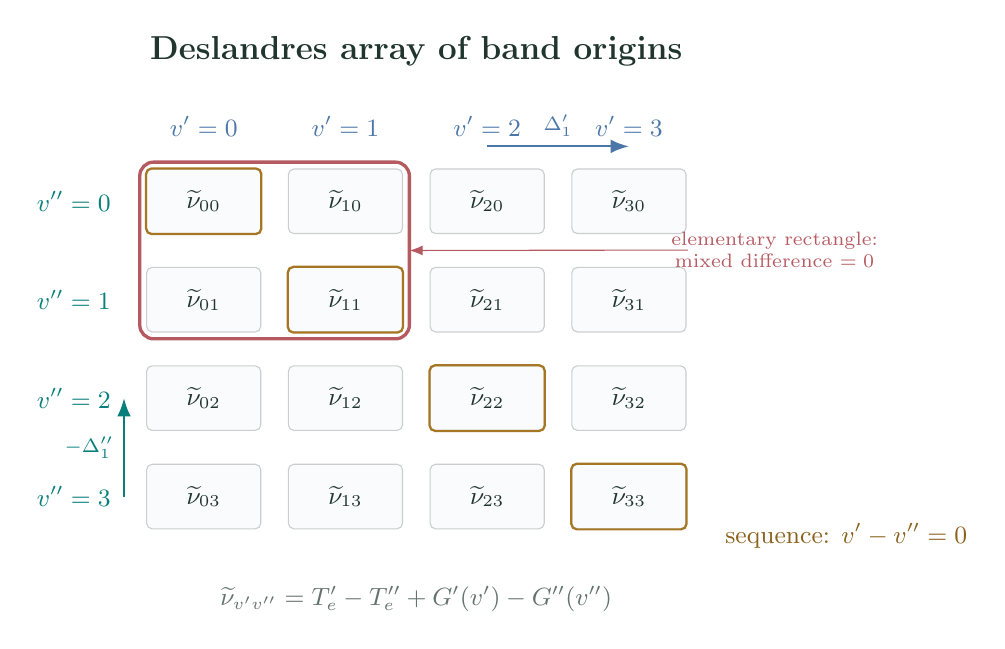
\begin{tikzpicture}[font=\sffamily,text=ink,>=Latex]
  \node[font=\bfseries\large] at (0,4.8)
    {Deslandres array of band origins};

  \foreach \i in {0,...,3}{
    \node[font=\small\bfseries,blue] at ({-2.7+1.8*\i},3.85)
      {$v'=\i$};
    \node[font=\small\bfseries,teal] at (-4.35,{2.9-1.25*\i})
      {$v''=\i$};
  }

  \foreach \i in {0,...,3}{
    \foreach \j in {0,...,3}{
      \pgfmathsetmacro{\xx}{-2.7+1.8*\i}
      \pgfmathsetmacro{\yy}{2.9-1.25*\j}
      \node[draw=ink!24,rounded corners=2pt,
            fill=blue!3,minimum width=1.45cm,
            minimum height=.82cm,font=\small]
        (c\i\j) at (\xx,\yy) {$\widetilde\nu_{\i\j}$};
    }
  }

  \draw[rose,very thick,rounded corners=5pt]
    ($(c00.north west)+(-.08,.08)$)--
    ($(c10.north east)+(.08,.08)$)--
    ($(c11.south east)+(.08,-.08)$)--
    ($(c01.south west)+(-.08,-.08)$)--cycle;
  \node[rose,font=\scriptsize,align=center] at (4.55,2.28)
    {elementary rectangle:\\mixed difference $=0$};
  \draw[rose,->] (3.45,2.28)--
    ($(c10.east)!.5!(c11.east)+(.08,0)$);

  \draw[blue,thick,->]
    ($(c20.north)+(0,.28)$)--($(c30.north)+(0,.28)$)
    node[midway,above,font=\scriptsize] {$\Delta_1'$};
  \draw[teal,thick,->]
    ($(c03.west)+(-.28,0)$)--($(c02.west)+(-.28,0)$)
    node[midway,left,font=\scriptsize] {$-\Delta_1''$};

  \foreach \i in {0,...,3}{
    \node[draw=gold!85!black,thick,rounded corners=2pt,
          fit=(c\i\i),inner sep=0pt] {};
  }
  \node[gold!70!black,font=\small,anchor=west] at (3.8,-1.35)
    {sequence: $v'-v''=0$};

  \node[font=\small,text=ink!70] at (0,-2.15)
    {$\widetilde\nu_{v'v''}=T_e'-T_e''+G'(v')-G''(v'')$};
\end{tikzpicture}
\end{document}
